% This version of CVPR template is provided by Ming-Ming Cheng.
% Please leave an issue if you found a bug:
% https://github.com/MCG-NKU/CVPR_Template.

%\documentclass[review]{cvpr}
\documentclass[final]{cvpr}

\usepackage{times}
\usepackage{epsfig}
\usepackage{graphicx}
\usepackage{amsmath}
\usepackage{amssymb}
\usepackage{multirow}

\usepackage{booktabs}
\usepackage{subcaption}

% Include other packages here, before hyperref.

% If you comment hyperref and then uncomment it, you should delete
% egpaper.aux before re-running latex.  (Or just hit 'q' on the first latex
% run, let it finish, and you should be clear).
\usepackage[pagebackref=true,breaklinks=true,colorlinks,bookmarks=false]{hyperref}

\def\cvprPaperID{****} % *** Enter the CVPR Paper ID here
\def\confYear{TODO}
%\setcounter{page}{4321} % For final version only

\begin{document}

%%%%%%%%% TODO because I don't know where else to put them
% TODO: put the source code to the paper to the repository - don't forget to remove the student IDs!
% TODO: export the paper and put it in the repository too, there is a link in the README to the PDF (paper/main.pdf)
% TODO: Create a new python env and run pip install -r requirements.txt and see if everything works or if we forgot something + commit the results // working on it

%%%%%%%%% TITLE
\title{Indoor Climbing Hold and Route Segmentation}

\author{
\begin{tabular}{c}% maybe change this formatting later
    Philipp Göldner, Kiryl Kisin, Tomáš Sláma \\
    Heidelberg University \\
    \\
\end{tabular}
}

\maketitle


\begin{abstract} % Tom
   Image segmentation has uses in a wide variety of fields, including medicine, geography, and sport.
   For indoor rock climbing specifically, the main task is the segmentation of the holds which the climbers use to scale the wall.
   Furthermore, since holds of the same color form routes, the secondary task is to find these routes.
   A number of approaches have been devised to solve these two tasks, with the two major categories being learning and non-learning approaches.
   We have tested and implemented both learning and non-learning (standard) approaches for these tasks, finding the learning approaches far superior in terms of accuracy, but less practical due to the need for good training data, which has to be obtained manually.
   The data, code and models were published free and open source.
\end{abstract}

\section{Introduction} % Tom
There has been an indisputable rise in popularity of indoor rock climbing, in no small part due to their inclusion in the Tokyo 2020 Summer Olympics.
With this rise comes an interest in interacting with climbing in a number of ways, a lot of which involve technology.

Computer vision, especially hold and route segmentation, can be used in commercial climbing gyms and competitions alike in a number of ways, namely
\begin{itemize}
    \item \textbf{competition judging} -- online pose recognition can be used to track the climber and measure how many times they attempted the climb and whether they reached the top, supplanting a need for a large team of judges
    \item \textbf{climbing journal} -- after a sector is rebuilt, the climbing gym can take images and, with the existence of a suitable mobile phone/web app, allow the climbers to interact with the routes by marking the ones they sent, liking/disliking, commenting and proposing grades (similar to apps that already exist for standardized boards like Kilterboard \cite{Kilterboard} and Moonboard \cite{Moonboard})
    \item \textbf{grade estimation} -- estimate the difficulty of a route in one of the standardized grading systems
\end{itemize}

Besides these specific use cases, any computer vision-related project that involves an indoor climbing gym will arguably need to determine which sections of images (or textures when dealing with 3D models) are holds and how they form routes. 

A number of the aforementioned tasks have already been attempted.
For grade estimation, a learning-based approach was developed \cite{MLRouteClassification} to infer the difficulty of the standardized Moonboard training board \cite{Moonboard}.
The competition judging was, to some extent, addressed by \cite{ClimbingAnalysis}, which performed post-climb analysis for climbers in commercial climbing gyms and also included standard and learning-based segmentation.
The segmentation tasks specifically were addressed by \cite{Climbnet,WeiDisplayer}, which used the standard and learning-based approaches respectively, but whose models and datasets are not freely available.


\section{Method}

Climbing gyms use holds and volumes of different shapes, sizes and colors in a variety of ways, the most common of which being the following: a single route is made up of holds of the same color, with the starting and ending holds denoted using colorful tape.
The volumes are large holds that are considered a part of the wall and so can be used while climbing any route, but change with every setting to make the structure of the wall less repetitive.

Working with these assumptions, the problem of hold segmentation can be formulated in the following way: given a 2D RGB image, output two sets of non-intersecting\footnote{This is a bit of a simplification, since a hold can be screwed on top of another hold (the same being true for volumes), but this arguably makes it a single structure, which greatly simplifies the task of segmentation.} polygons that determine the locations of the holds and volumes in the image.

Similarly, route segmentation can be formulated in the following way: given images of holds (which can be obtained from hold segmentation), output sets of holds that form different routes.
An important note to be made here is that since volumes are a part of every route, they can be safely ignored, which somewhat simplifies the problem.
While this is not always the case and there are gyms that use volumes for specific routes only, the common approach is to allow their usage for every route. 


\subsection{Obtaining data}\label{sec:obtaining_data}  % Tom
For training and testing the methods, three datasets were acquired across two climbing gyms~--~Smíchoff (Czech Republic) and Boulderhaus (Heidelberg).
To compare the behavior of the methods on different image quality, two devices were used -- a modern DLSR camera and a modern smartphone. The parameters of the dataset are denoted in \autoref{tab:dataset}.

% https://www.tablesgenerator.com/#
\begin{table}[h]
\centering
\begin{tabular}{@{}llrr@{}}
\toprule
Location & Device & Images & Annotated \\ \midrule
Boulderhaus       & Nikon Z 50         & 1062           & 15 hold (8 route)           \\
Boulderhaus       & Samsung A51 & 244            & 2 hold (0 route)           \\
Smíchoff          & Nikon Z 50         & 972            & 2 hold (0 route)           \\ \bottomrule
\end{tabular}
\caption{Dataset parameters.}
\label{tab:dataset}
\end{table}

Having access to images from more than one climbing gym is important, since while the general concept of "holds on a wall" is the same, the gyms have holds from different manufacturers and also different backgrounds (dark/light), as seen in \autoref{fig:sm-v-bg}.

\begin{figure}[h]
\centering
\begin{subfigure}{0.49\linewidth}
\centering
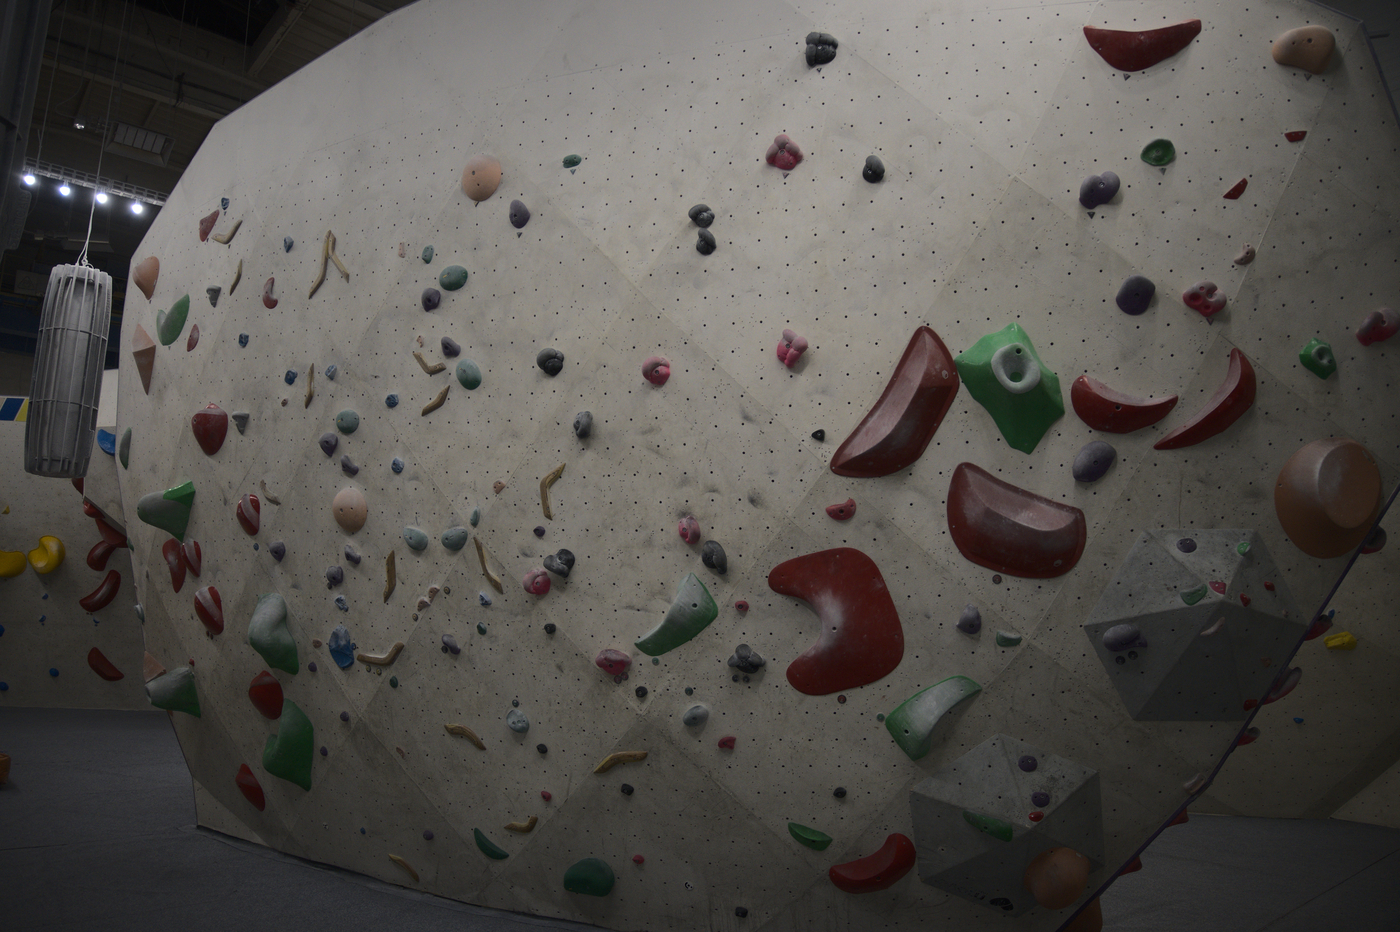
\includegraphics[width = \linewidth]{img/sm.jpg}
\caption{Smíchoff image}
\end{subfigure}
\begin{subfigure}{0.49\linewidth}
\centering
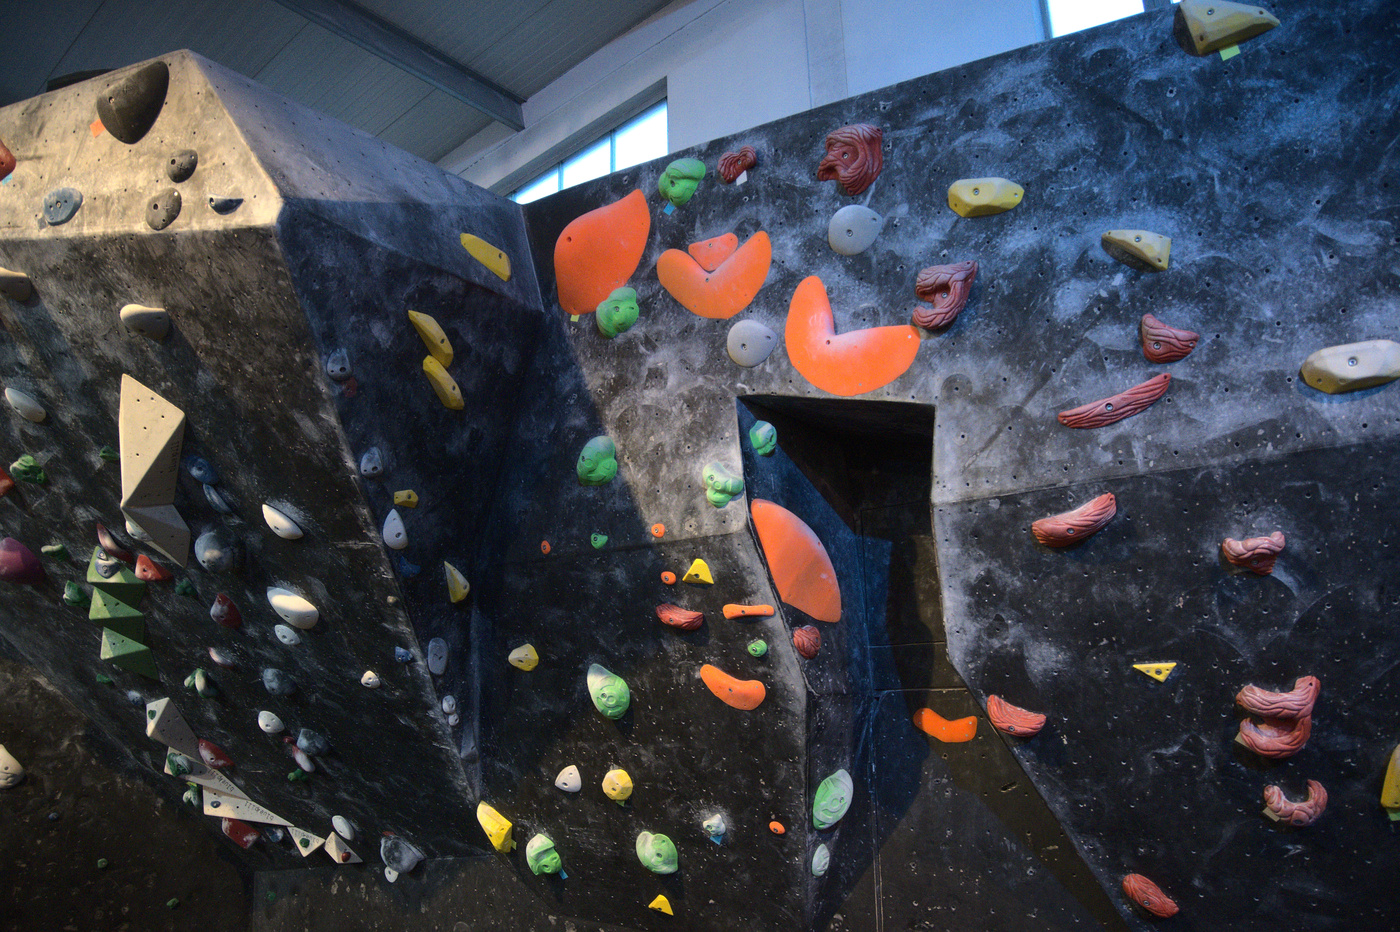
\includegraphics[width = \linewidth]{img/bh.jpg}
\caption{Boulderhaus image}
\end{subfigure}
\caption{Smíchoff and Boulderhaus comparison.}
\label{fig:sm-v-bg}
\end{figure}

For benchmarking and training learning-based methods, a certain subset of the images had to be manually annotated.
To achieve this, the VGG Image Annotator (VIA) \cite{dutta2016via,dutta2019vgg} was used on a subset of images from each of the respective datasets with varying numbers and sizes of holds and volumes, lighting conditions, perspectives, background, etc.
Each hold outline was approximated with a polygon and labeled as either a hold or a volume.
Holds that formed routes were assigned the same route ID.

% Tom: not referenced, removing for now at least
%\begin{figure}[h]
%\centering
%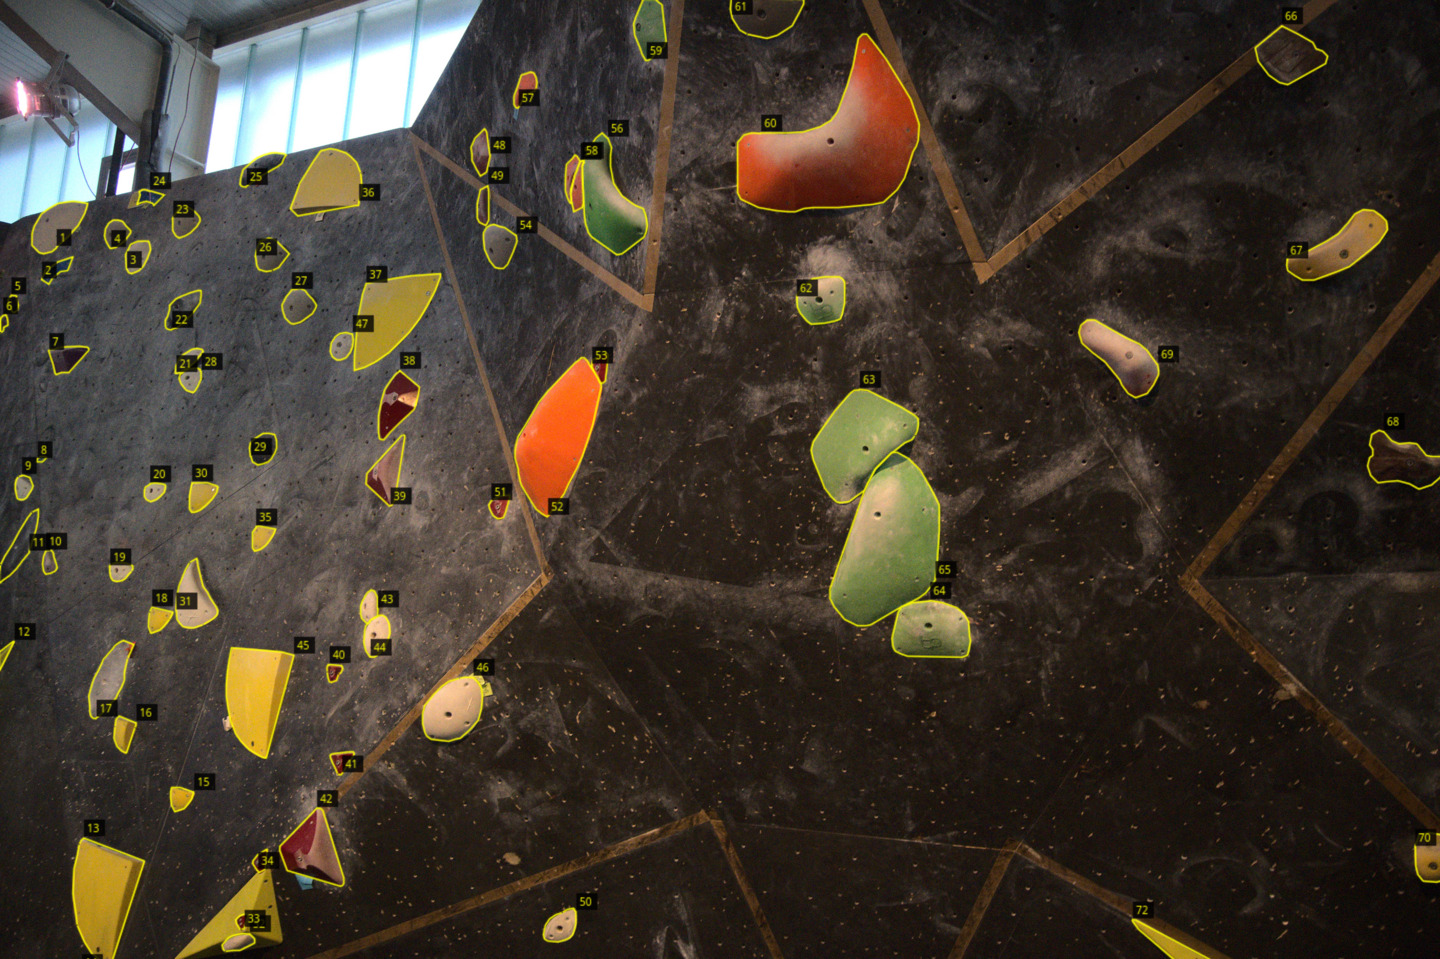
\includegraphics[width = \linewidth]{img/dataset-sample-3.jpg}
%\caption{sample annotated image (Boulderhaus)}
%\label{fig:sample-dataset-image}
%\end{figure}

Across all of the datasets, a total of 1688 shapes were manually annotated, split 1597/91 for holds/volumes.
The sizes of the annotations (wrt. percent of image size) and numbers per-image can be seen in \autoref{fig:instance-size} and \ref{fig:instance-per-category}.

\begin{figure}[h]
\centering
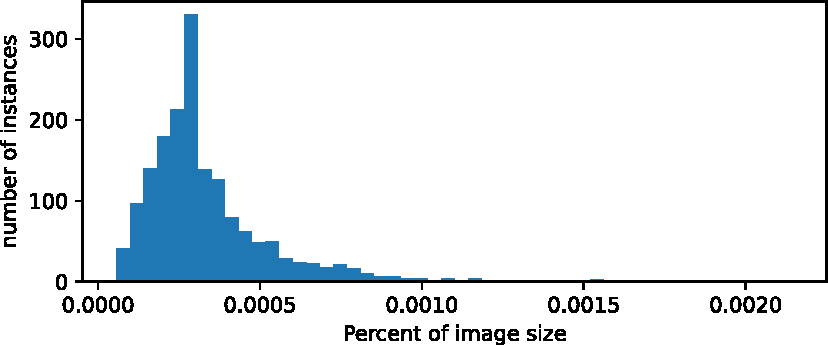
\includegraphics[width = \linewidth]{img/statistics/instance_size.pdf}
\caption{Hold size wrt. percent of image size.}
\label{fig:instance-size}
\end{figure}

\begin{figure}[h]
\centering
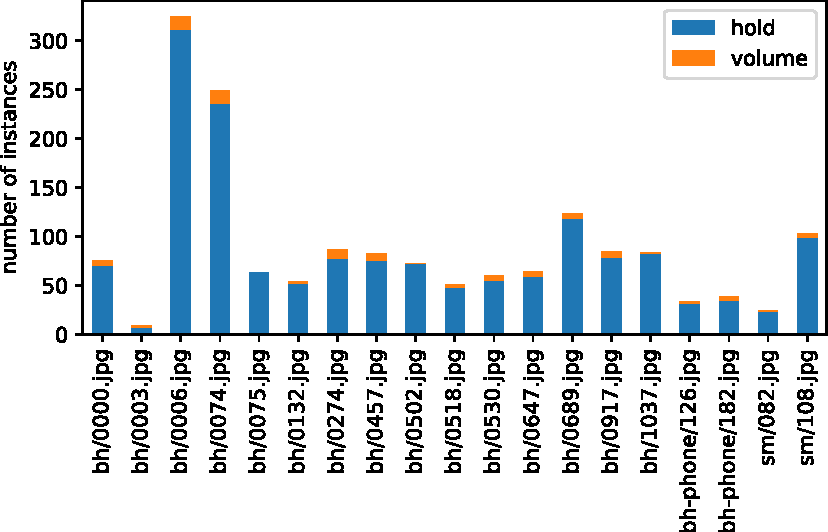
\includegraphics[width = \linewidth]{img/statistics/instances_per_category.pdf}
\caption{Number of hold/volume instances per category.}
\label{fig:instance-per-category}
\end{figure}

The datasets, including both the images and the annotations, were made freely available under the CC NC-SA 4.0 license via Kaggle \cite{Our}.

\subsection{Hold segmentation} % Tom

\subsubsection{Standard approach} % Tom

From the perspective of a standard approach, there are two main things that define a hold: edges and color.
Unfortunately, they also define a number of other objects in the scene, which is a major drawback of this method~--~there is no easy way to determine the semantics of an object.

Both of the approaches were implemented and tested on the datasets using Python and OpenCV \cite{opencv}.
They are inspired by \cite{ClimbingAnalysis}, which also discusses blob and edge detection, but are improved upon by using a number of hold-specific heuristics and implementing the hold detection via the combination of the two.

For edge detection, the Canny edge detector was used (hysteresis thresholds $20$, $25$) on a Gaussian-blurred image for reducing edge noise.
To remove unwanted edges (namely bolt holes), the edges were filtered based on the minimal area they cover.
They are additionally filtered based on their straightness for removing seams in the wall, which was done by linear regression of the edge points and subsequent filtering based on the average squared distance of the points to the regressed line.
Results on a sample image can be seen in \autoref{fig:edges}.

\begin{figure}[t]
\centering
\begin{subfigure}{0.49\linewidth}
\centering
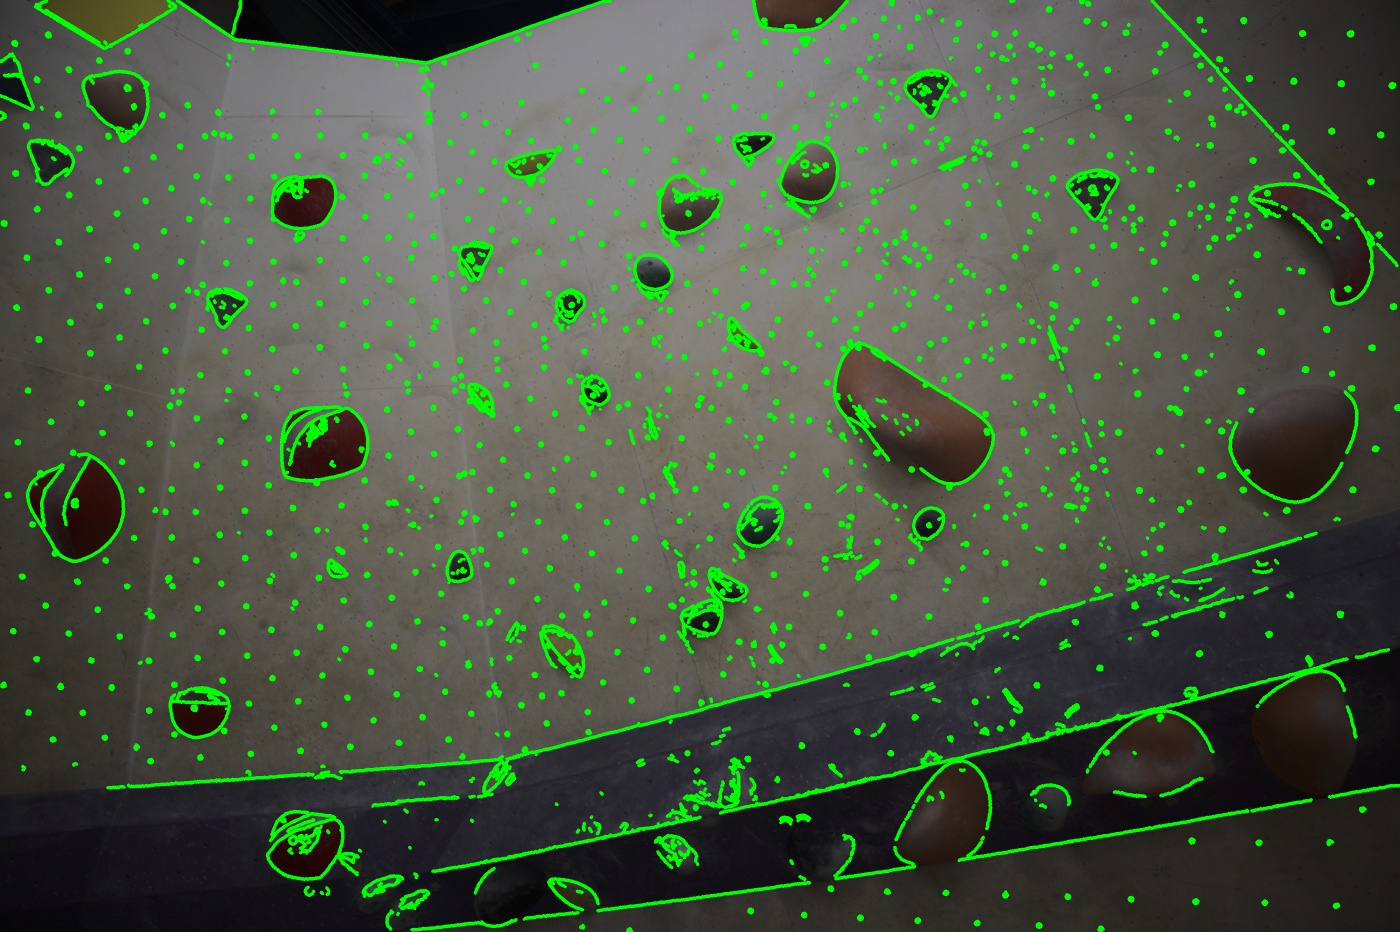
\includegraphics[width = \linewidth]{img/edges/4-contours.jpg}
\caption{Canny edge detection}
\label{fig:edges:a}
\end{subfigure}
\begin{subfigure}{0.49\linewidth}
\centering
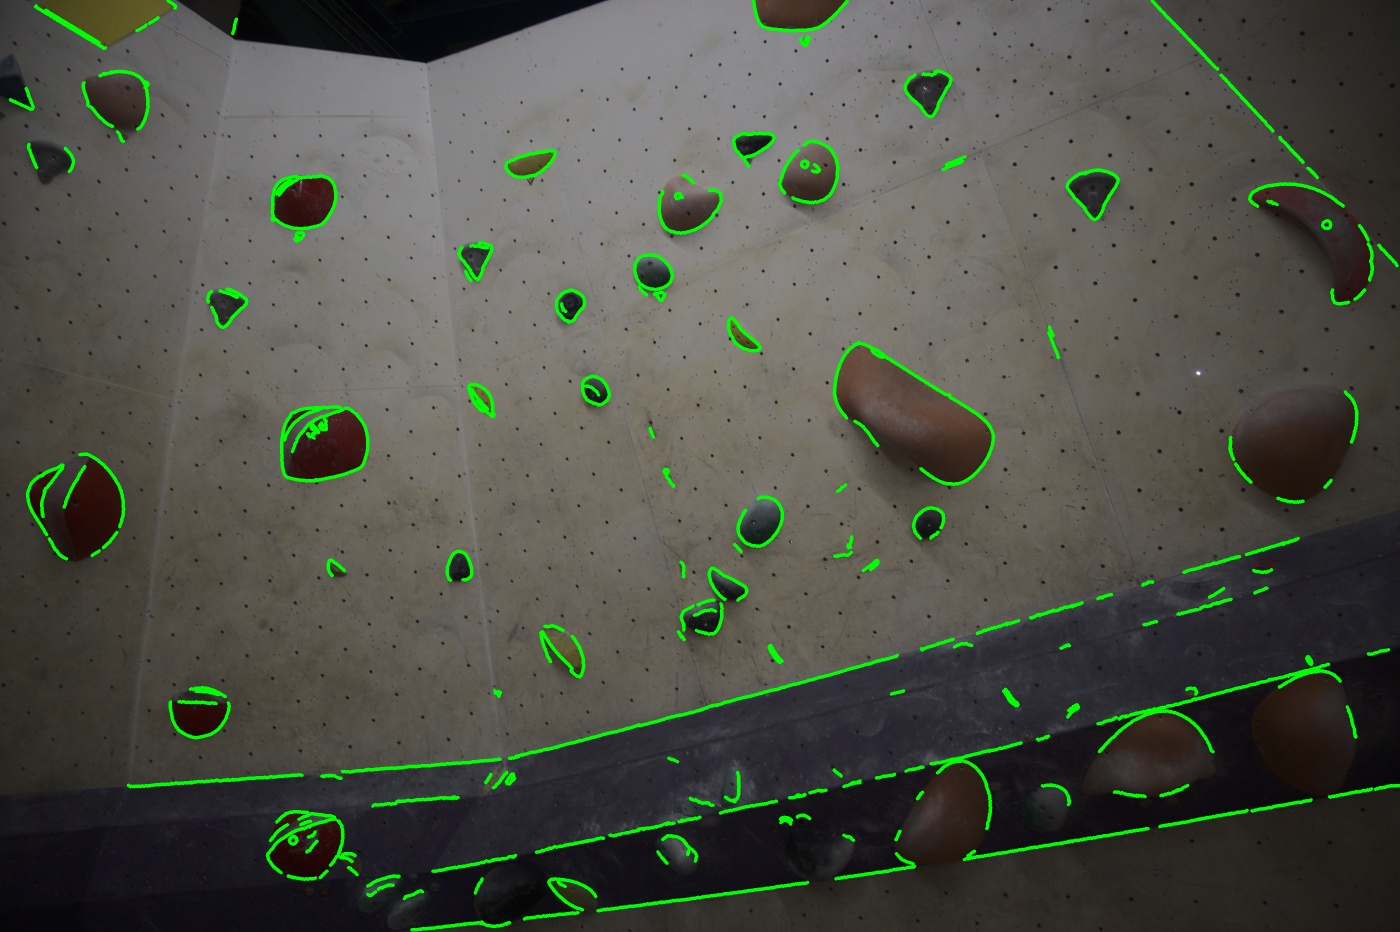
\includegraphics[width = \linewidth]{img/edges/5-contours-area-filter.jpg}
\caption{area filtering}
\label{fig:edges:b}
\end{subfigure}
\\[0.5em]
\begin{subfigure}{1\linewidth}
\centering
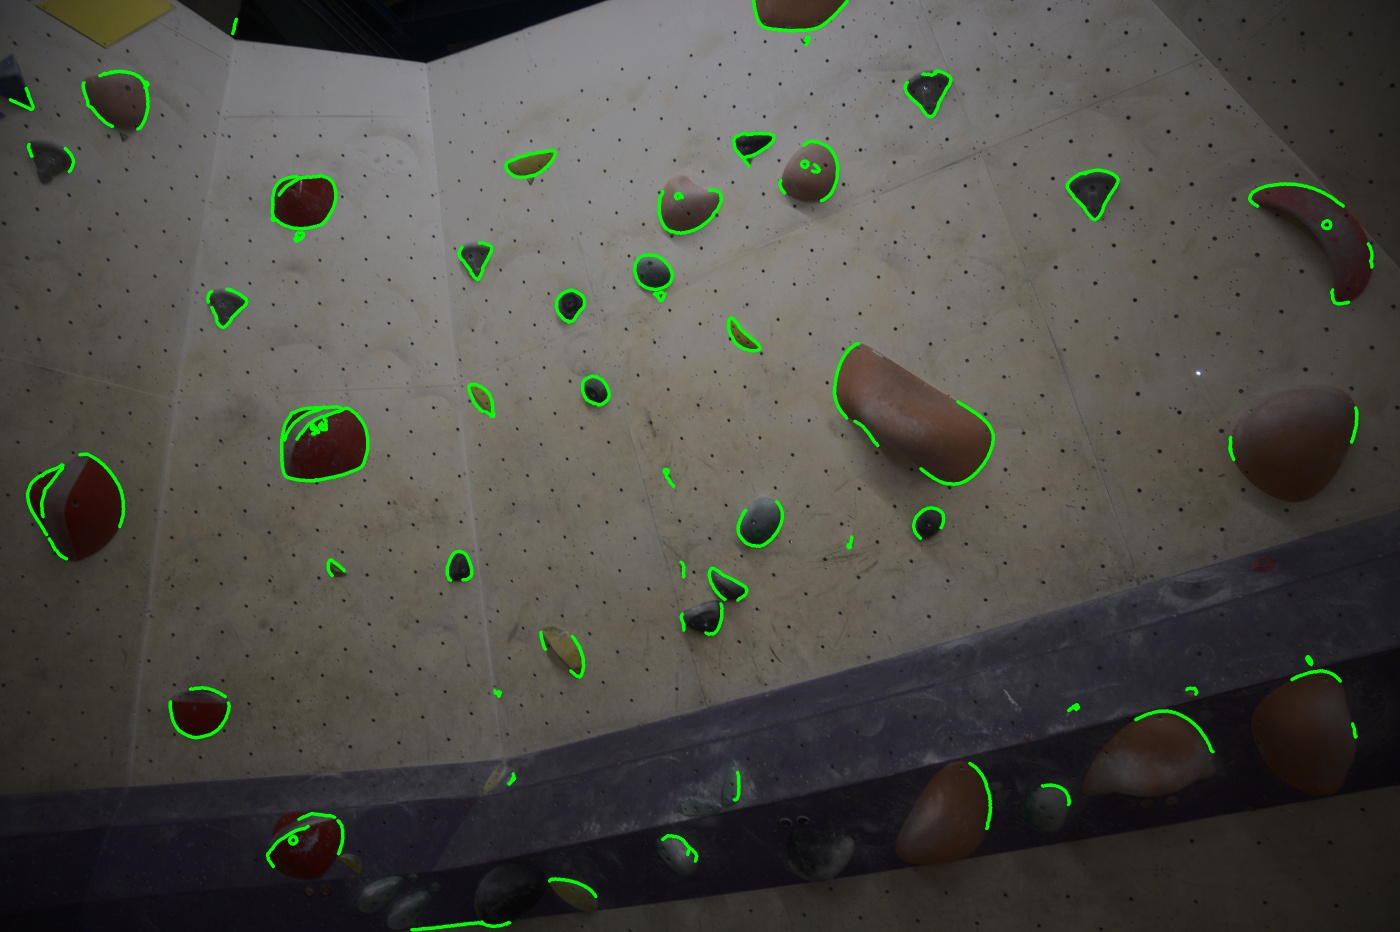
\includegraphics[width = \linewidth]{img/edges/6-contours-straight-filter.jpg}
\caption{straightness filtering}
\label{fig:edges:c}
\end{subfigure}
\caption{Standard edge detection.}
\label{fig:edges}
\end{figure}

\begin{figure}[b]
\centering
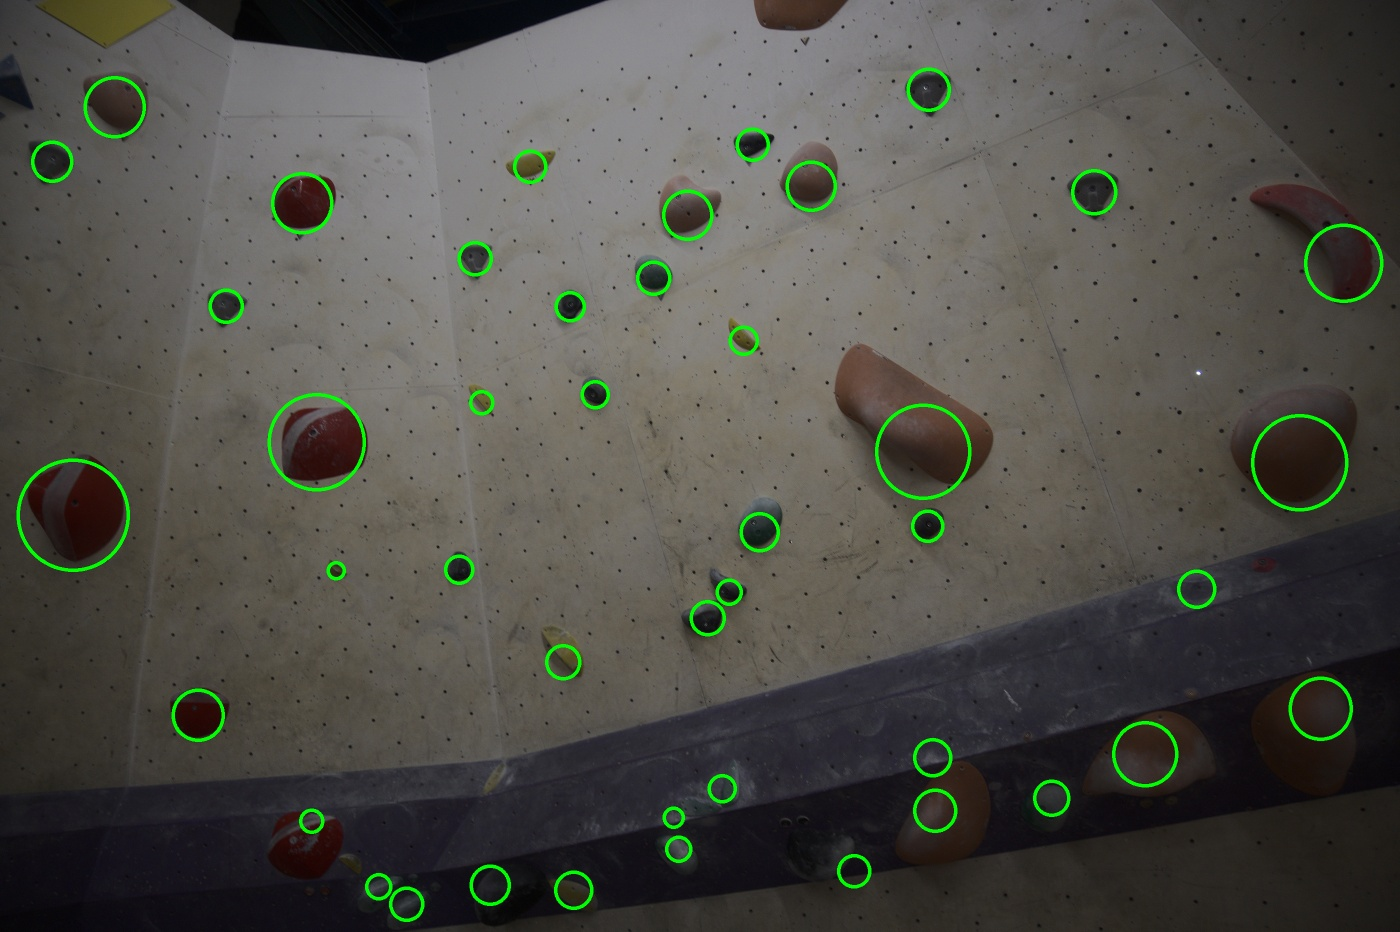
\includegraphics[width = \linewidth]{img/blobs/3-blobs-merged.jpg}
\caption{Standard blob detection.}
\label{fig:blobs}
\end{figure}

For blob detection, the simple blob detector was used with filtering by area.
It works by converting the source image to binary using various brightness thresholds (min $1$, max $200$, step $10$ was used), extracting the centers of their connected components and grouping centers that are close to one another into single blobs.
Additionally, blobs with large overlap (over $15\%$) were merged~--~this is a common occurrence for dual-texture holds, since white chalk only sticks to the rough texture and thus visually splits the hold.
Results on a sample image can be seen in \autoref{fig:blobs}.

These two approaches can be combined in a straightforward way~--~detected blobs are locations of holds and edges are guides for their outlines.
To refine these outlines into a hold mask, binary thresholds of the image for a certain step size can be taken (in the RGB channels respectively).
The Canny edge detector can then be used on the threshold image for each step size, picking the contour that is the closest to the original outline given an appropriate metric (the squared sum distance of points from one contour to the other, for example).
Results on a sample image can be seen in \autoref{fig:holds}.

\begin{figure}[t]
\centering
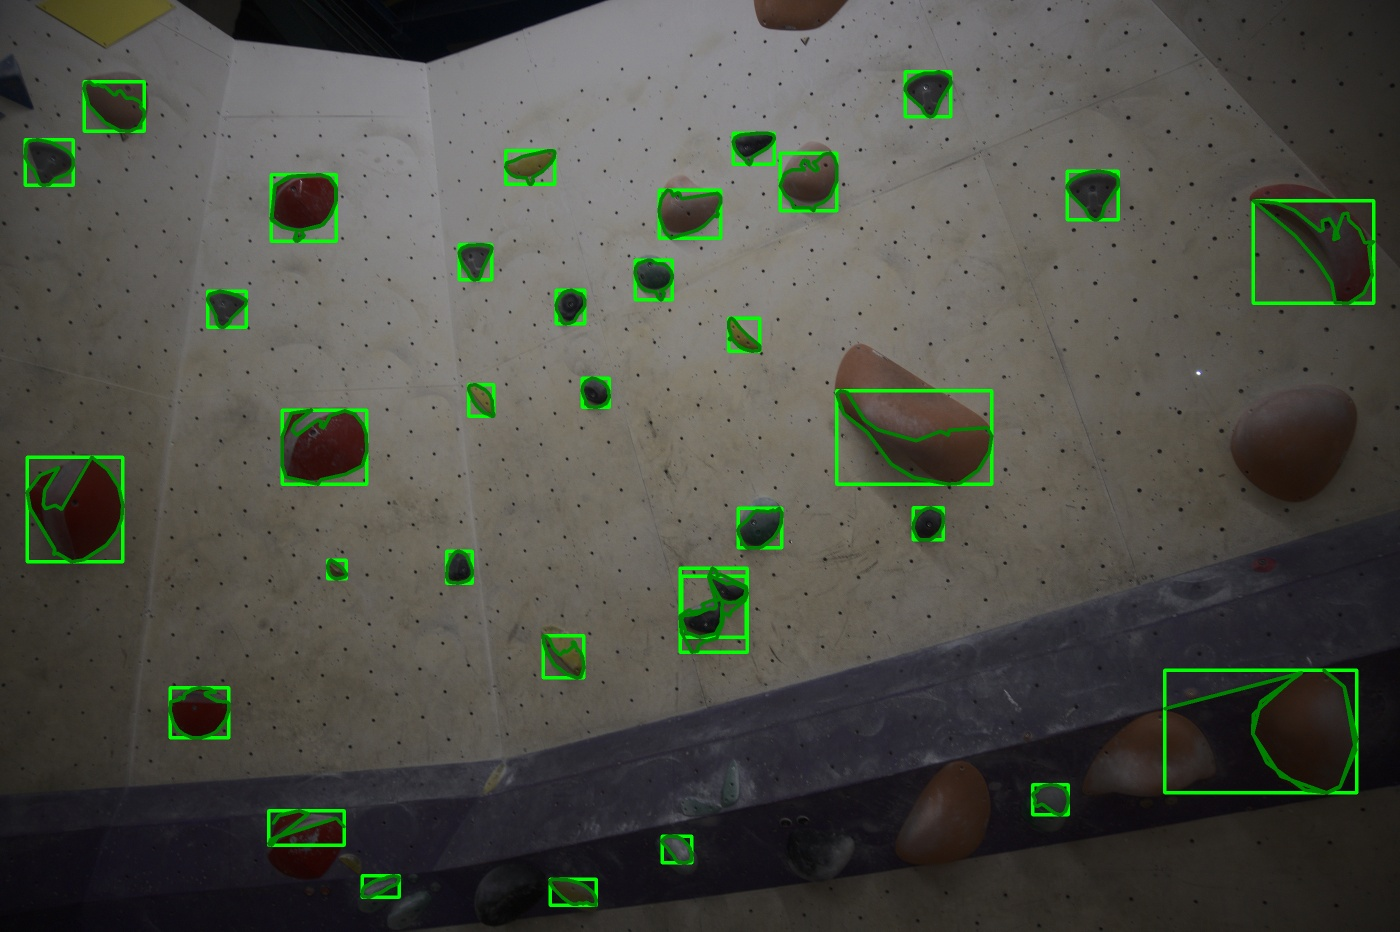
\includegraphics[width = \linewidth]{img/combined/2-holds.jpg}
\caption{Standard hold detection.}
\label{fig:holds}
\end{figure}

Another major drawback of this method is that the optimal parameters of both the edge and blob detection are different for each input image.
To remedy this, a portion of the parameters can be estimated using various heuristic functions -- filtering of blobs and contours based on minimal blob/contour area can be set such that the area must be larger than the size of the bolt holes in the walls (see \autoref{fig:edges:a}), which can be determined as a spike in the histogram over the area of all contours.
It is, however, problematic to do so for every dataset, since some (especially competition) walls, like a subset of images from the Smíchoff dataset, may not include bolt holes at all.

\begin{table*}[t!]  % NOTE: this doesn't belong here but I can't make LaTeX place the figure correctly otherwise
    \centering
    \begin{tabular}{lp{11cm}} % hack
           \toprule
         Model name & Description  \\\midrule
         Basic & default parameters, no augmentations \\
         Augmented & augmentations \\
         Augmented-NoRandomCrop & augmentations without RandomCrop \\
         Augmented-DoubleTopK-NMS & augmentations, double default number of top-k results pre and post NMS \\
         Augmented-P2P3 & augmentations, $P_2$/$P_3$ features as input for ROI head and segmentation head\\
         Augmented-P2P3-DoubleTopK-NMS & augmentations, $P_2$/$P_3$ features as input for ROI head and segmentation head,  double default number of top-k results pre and post NMS\\
         Augmented-P2P3-DoubleTopK-NMS-2K & same as Augmented-P2P3-DoubleTopK-NMS but trained for 2000 iterations\\ \bottomrule
         
    \end{tabular}
    \caption{Description of different models for hold detection.}
    \label{tab:model_descriptions}
\end{table*}

\begin{figure*}[t!]  % NOTE: this doesn't belong here but I can't make LaTeX place the figure correctly otherwise
\centering%
\begin{subfigure}{0.488\linewidth}%
\centering%
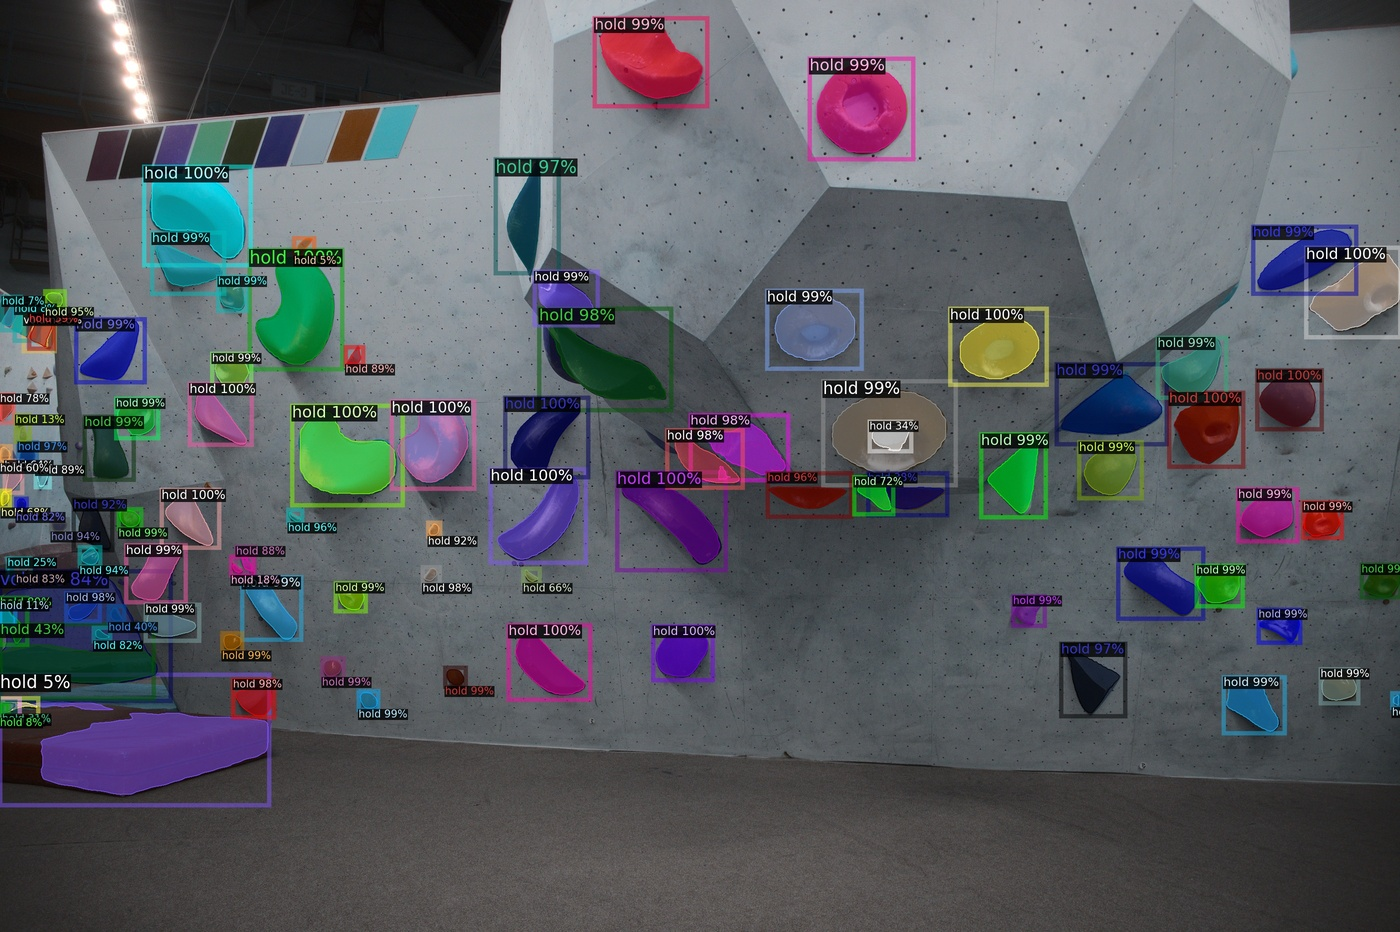
\includegraphics[width = \linewidth]{img/converted-sm-image.jpg}%
\caption{Smíchoff image}%
\end{subfigure}\quad
\begin{subfigure}{0.488\linewidth}%
\centering%
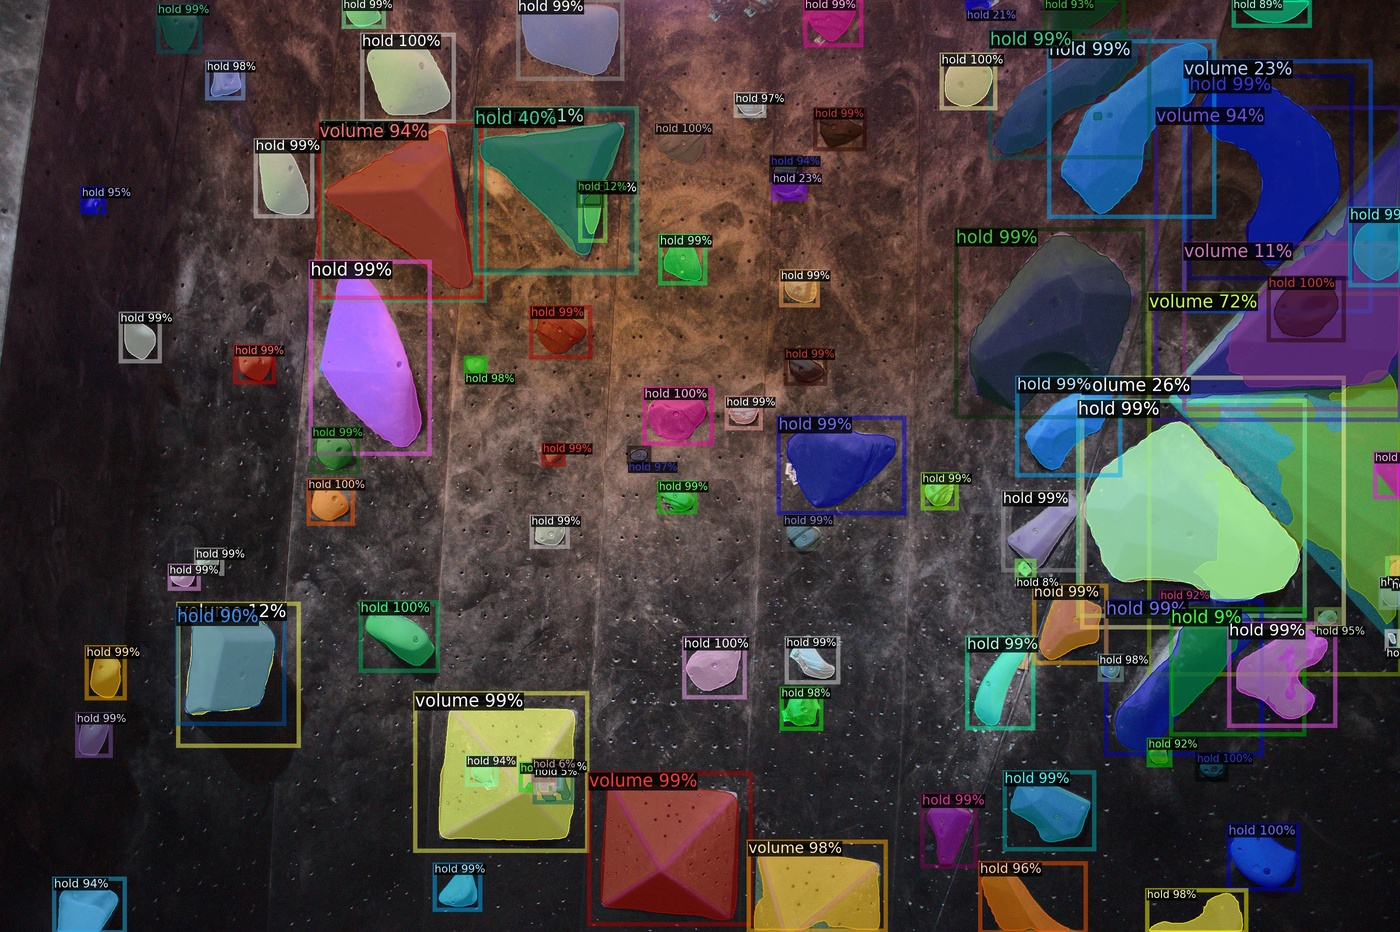
\includegraphics[width = \linewidth]{img/converted-bh-image.jpg}%
\caption{Boulderhaus image (camera)}%
\end{subfigure}
%\begin{subfigure}{0.345\linewidth}%
%\centering%
%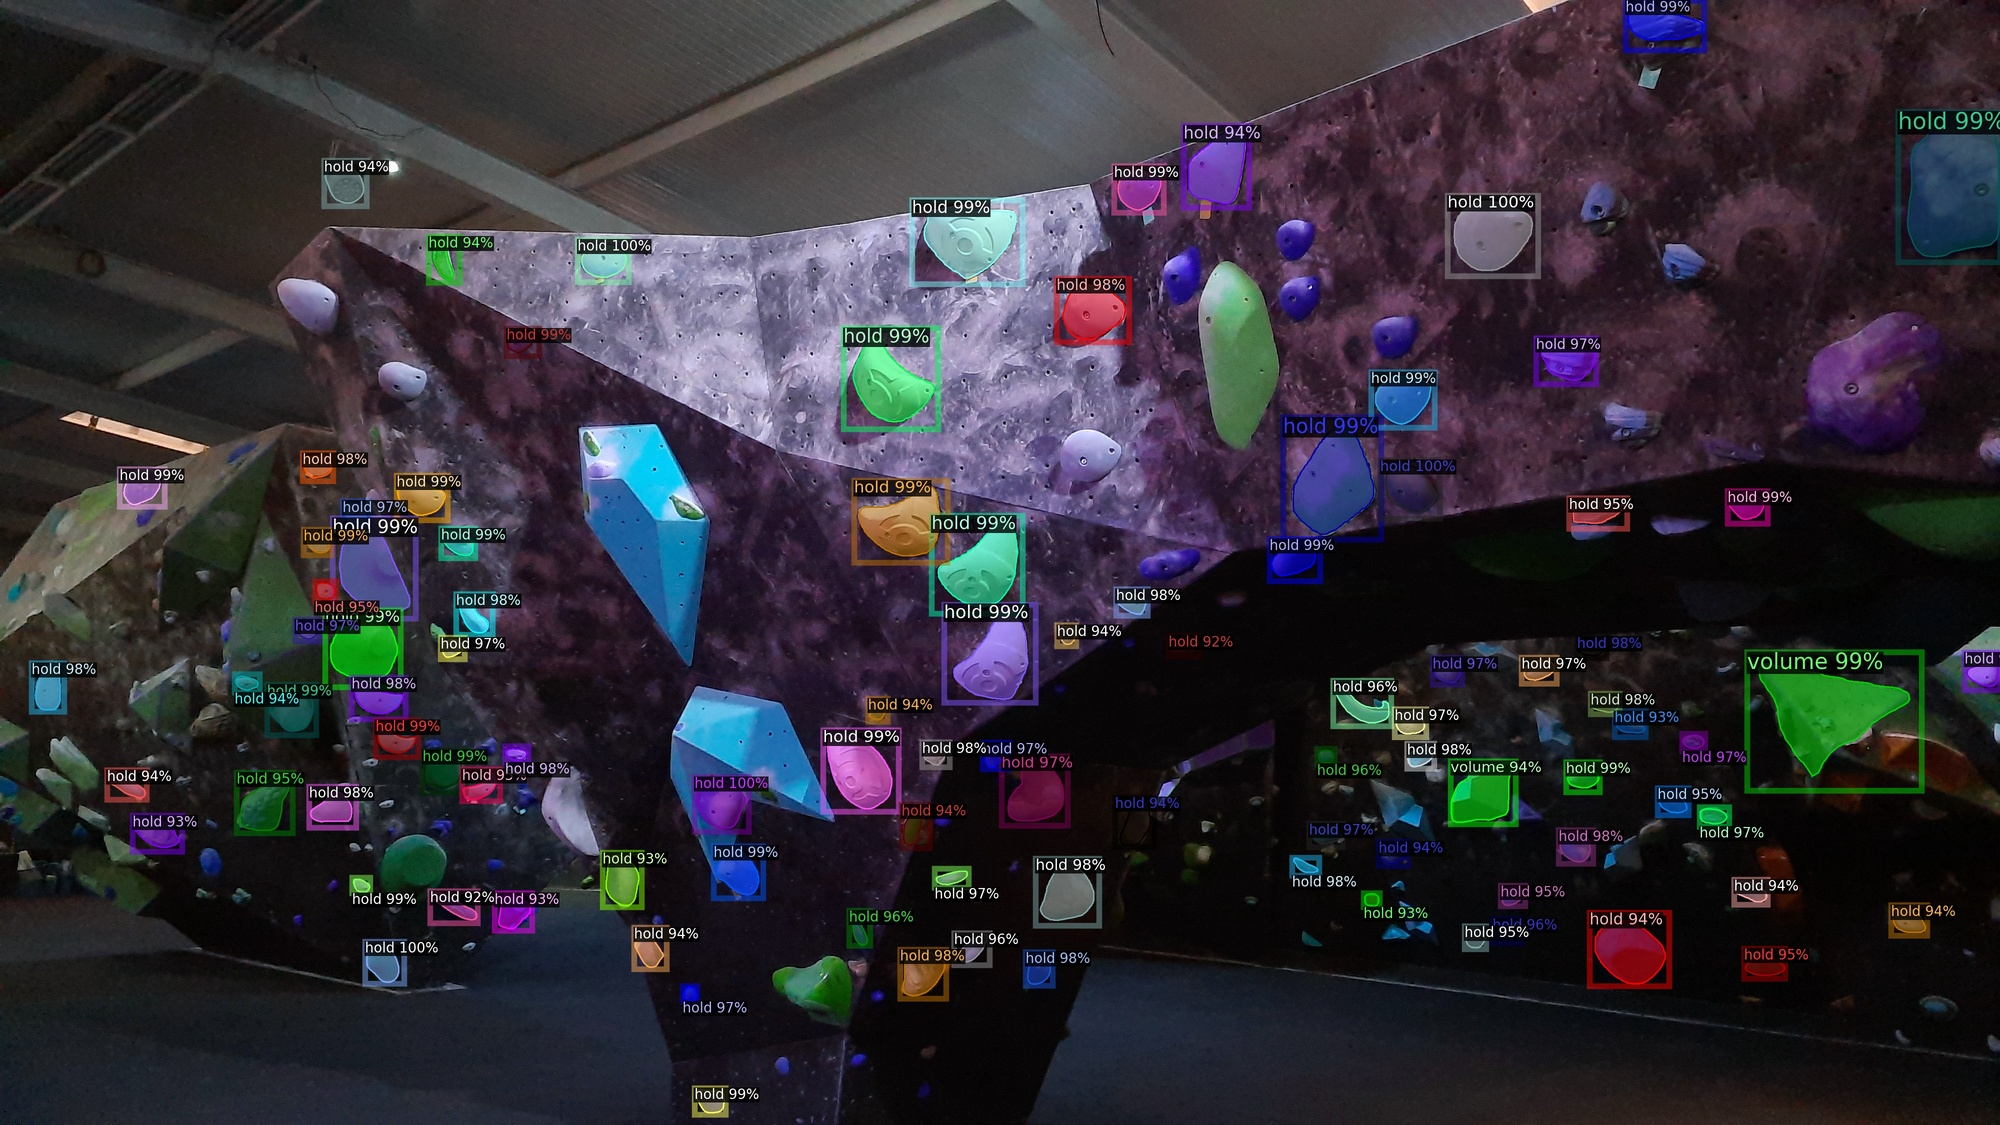
\includegraphics[width = \linewidth]{img/converted-phone-image.jpg}%
%\caption{Boulderhaus image (phone)}%
%\end{subfigure}%
\caption{Results of Augmented-P2P3-DoubleTopK-NMS-2K on two images from the testing dataset.}%
\label{fig:results-sm-bh}%
\end{figure*}

For images that require even slightly different parameters (the method assumes a light background and dark holds), the method produces results that are entirely wrong, both in terms of false positives and false negatives.
It serves as a proof of concept and not a viable alternative to learning-based hold segmentation, as discussed in \autoref{sec:conclusion}.


\subsubsection{Learning-based approach} % Philipp


\begin{table*}[t!]  % NOTE: this doesn't belong here but I can't make LaTeX place the figure correctly otherwise
    \centering
    \begin{tabular}{llrrr}
        \toprule
         Dataset & Model Name & mAP & \textbf{AP hold} & AP volume  \\\midrule
         \multirow{7}{*}{Boulderhaus} & Basic & 54.59 & 57.84 & 51.33 \\
                                     & Augmented & 52.28 & 64.62 & 39.94 \\
                                     & Augmented-NoRandomCrop & 59.70 & 62.82 & 56.57 \\
                                     & Augmented-DoubleTopK-NMS & 54.41 & 65.04 & 43.78 \\
                                     & Augmented-P2P3 & 39.51 & 37.96 & 41.05 \\
                                     & Augmented-P2P3-DoubleTopK-NMS & 57.05 & 62.61 & 51.49 \\
                                     & Augmented-P2P3-DoubleTopK-NMS-2K & \textbf{62.28} & \textbf{65.99} & \textbf{58.56} \\
        \hline
        \multirow{7}{*}{Boulderhaus-Phone} & Basic & 74.16 & 74.63 & 73.69 \\
                                        & Augmented & 71.59 & 80.84 & 62.33 \\
                                        & Augmented-NoRandomCrop & 77.38 & 78.88 & 75.88 \\
                                        & Augmented-DoubleTopK-NMS & 76.86 & \textbf{81.23} & 72.49 \\
                                        & Augmented-P2P3 & 60.66 & 61.52 & 59.80 \\
                                        & Augmented-P2P3-DoubleTopK-NMS & \textbf{78.00} & 79.89 & \textbf{76.11} \\
                                        & Augmented-P2P3-DoubleTopK-NMS-2K & 72.80 & 80.85 & 64.75 \\
        \hline
        \multirow{7}{*}{Smíchoff} & Basic & 37.57 & 58.30 & 16.83 \\
                                        & Augmented & 38.02 & 59.22 & 16.83 \\
                                        & Augmented-NoRandomCrop & 39.21 & 61.59 & 16.83 \\
                                        & Augmented-DoubleTopK-NMS & 35.34 & 62.26 & 8.42 \\
                                        & Augmented-P2P3 & 29.29 & 41.74 & 16.83 \\
                                        & Augmented-P2P3-DoubleTopK-NMS & 39.12 & 61.40 & 16.83 \\
                                        & Augmented-P2P3-DoubleTopK-NMS-2K & \textbf{40.25} & \textbf{63.67} & \textbf{16.83} \\ \bottomrule
                                     
    \end{tabular}
    \caption{ Evaluation results for different models and datasets. AP at IoU=.50:.05:.95.}
    \label{tab:results_hold_detection_ml}
\end{table*}


For the learning-based approach, we used the Mask R-CNN \cite{maskrcnn} architecture.
Specifically, the implementation from the detectron2 \cite{wu2019detectron2} library was used, because it provides simple training abstractions with sane default values. Furthermore, the library provides many useful helper functions for working with custom datasets and visualizing segmentation results.
The authors of the detectron2 library provide the weights for a number of pretrained models in their model zoo\footnote{Available at \url{https://github.com/facebookresearch/detectron2/blob/main/MODEL_ZOO.md}.}.
We used the \texttt{mask\_rcnn\_R\_50\_FPN\_3x} model weights which were trained on the large-scale segmentation dataset COCO \cite{coco} and further fine-tuned this model to our specific segmentation task.

Since our dataset size is quite limited, we relied on data augmentations to make our model more robust and generalize better.
We start by randomly cropping a region of $(0.5 * \texttt{height}, 0.5 * \texttt{width})$ from the image. This region is resized so that the short edge is 640 pixels.
The image is then randomly flipped horizontally and small random rotation, brightness, contrast and saturation changes are applied to the image.

We split the dataset into a train dataset (80\%) and a test dataset (20\%).
We trained multiple versions of this model. If not indicated otherwise, all the models were trained for 1000 iterations on a GTX 1060 6GB with a learning rate $\epsilon=0.0006$ and default parameters from the \texttt{mask\_rcnn\_R\_50\_FPN\_3x} model configuration.

Our dataset is very different from COCO, not only because it contains hundreds of instances per image, but also because these instances only occupy a small percentage of the total image size.
Therefore, we experimented with tuning different parameters of the model to make it detect more instances per image and also improve the performance on detecting smaller objects.

In our first experiment we doubled the number of top-k results that are generated by the region proposal network (RPN) (before non-maximum suppression (NMS) from 12000 to 24000, while also doubling the number of top-k results that are kept after performing NMS from 2000 to 4000. This allows the model to detect more instances per image.
For our second experiment, we wanted to improve the performance of the model on small objects. 
Mask R-CNN uses a feature pyramid network (FPN) \cite{FPN} to obtain features at different scales and aspect ratios for a single-scale input image.
This is generally of advantage because it allows the model to detect small and large objects in an image. For our application we only need to detect small objects in an image, which is why we modified the semantic segmentation head and the region-of-interest (ROI) head of the Mask R-CNN model to only use the $P_2$ (features from image at $1/4$ scale) and $P_3$ (features from image at $1/8$ scale) features.

In total, we trained seven variations of the model with different augmentation strategies and different combinations of these parameters. The different models are described in \autoref{tab:model_descriptions}.


For testing, we increased the maximum number of detections per image to 300.
The model is evaluated by calculating the intersection over union (IoU) between the predicted masks ($\text{mask}_{p}$) and the ground truth masks ($\text{mask}_{gt}$).
$$\mathrm{IoU} = \frac{\text{area}(\text{mask}_{p} \cap \text{mask}_{gt})}{\text{area}(\text{mask}_{p} \cup \text{mask}_{gt})}$$
If the IoU value is larger than a certain threshold $t$ and the class was correctly predicted, it is considered a true positive (TP) otherwise a false positive (FP).
The average precision (AP) is then calculated using the area under the curve (AOC) of the precision-recall curve.
This is repeated for each class $K$ to calculate the mean average precision (mAP), resulting in the following equation:
$$\mathrm{mAP} = \frac{1}{|K|} \sum_{i = 1}^{|K|} \mathrm{AP}_i$$
For calculating the final metric, we repeat this process at different IoU thresholds $t \in T=\{0.50, 0.55, ..., 0.95\}$ and calculate the mean.
This is the same metric that is used on the COCO \cite{coco} dataset.
The results of the evaluation can be seen in \autoref{tab:results_hold_detection_ml}.


As we have seen in \autoref{sec:obtaining_data}, we only have a small number of volumes in the dataset, so the mAP and AP-volume metrics are not really meaningful.
We therefore only look at the AP-hold metric for this comparison.
The \texttt{Augmented-P2P3-DoubleTopK-NMS-2K} performed best on the Boulderhaus and Smíchoff dataset, with an average precision of 65.99 and 63.67 respectively. It is very surprising that the model performs only slightly worse on the Smíchoff dataset, considering that the walls are light instead of dark like in the Boulderhaus dataset. This shows that the model can generalize well and can detect holds independent of the color of wall it was trained on.

On the Boulderhaus-Phone dataset, the best performing model was \texttt{Augmented-DoubleTopK-NMS}, with an average precision of 81.23. The other models also have a significantly higher AP score on this dataset compared to the Boulderhaus and Smíchoff datasets. This is likely the case because images were taken much closer to the wall, and therefore the holds are much larger and easier to segment. This could also explain why the \texttt{Augmented-P2P3-DoubleTopK-NMS-2K} model does not perform as well on this dataset, because it was optimized to detect small objects on the wall.

An example of the resulting bounding boxes and segmentation masks can be seen in \autoref{fig:results-sm-bh}. We can see that the model performs really well on creating bounding boxes and segmentations masks for holds, but struggles with segmentation masks for volumes. This can be explained by the limited number of volumes in our training set (63 volumes compared to 1214 holds). Similarly, the model struggles with the edge case where holds are mounted on top of a volume instead of on the wall, which is a relatively rare occurrence in the training set.



\subsection{Route segmentation}

\subsubsection{Standard approach} % Kiryl 
After holds were found and annotated, we started forming routes from holds of same colors. For the standard approach, we used the OpenCV library \cite{opencv} and k-means and k-medoids clustering from the scikit-learn module \cite{scikit} with different feature sets. Since these clustering techniques are similar, they gave us pretty close results.

\begin{figure}[h]
\centering

\includegraphics[width = \linewidth]{img/routes_std/red_holds.jpg}
\caption{Mean RGB colors. Red route.}
\label{fig:red_route}
\end{figure}

There are several possible feature sets that could combine holds of same colors into routes. The first one is a set of mean RGB colors \cite{meancolorclustering} representing each hold, which stores mean color values calculated for each color channel from every pixel of one hold. RGB color featuring allowed the algorithm to perform well when images were bright and clear (no shadows or chalk spots), clustering holds with similar enough colors as one route. Clustering results in \autoref{fig:red_route} illustrate that ten out of twelve red holds were annotated correctly and one was labeled as false positive. Unfortunately, the algorithm accuracy was not high, when some clusters contain several different routes (see \autoref{fig:bad_cluster}).

\begin{figure}[h]
\centering

\includegraphics[width = \linewidth]{img/routes_std/bad_cluster.jpg}
\caption{Mean RGB colors. Wrong result.}
\label{fig:bad_cluster}
\end{figure}

Another set of features was color moments. Color moments characterize image color distribution similarly to how central moments uniquely describe a probability distribution. An algorithm with color moment features produced less false positives but was prone to assign holds of the same color to different clusters, as shown in \autoref{fig:several_clusters}.

\begin{figure}[h]
\centering
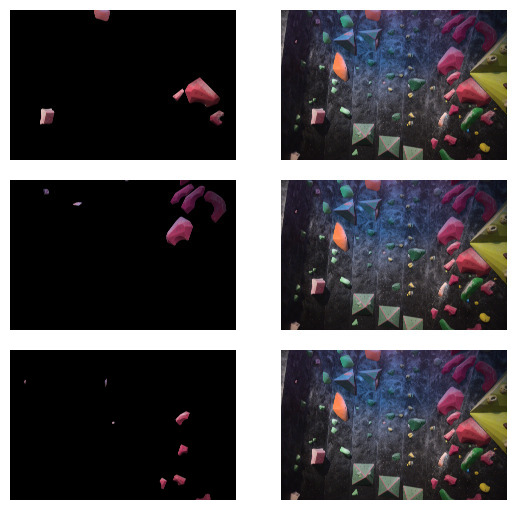
\includegraphics[width = \linewidth]{img/routes_std/several_clusters.jpg}
\caption{Color moments. Multiple red routes.}
\label{fig:several_clusters}
\end{figure}

Histograms can also aid hold featuring. For our problem, we used OpenCV's calcHist function to calculate histograms of all three RGB channels for each hold. Surprisingly, the clustering result was worse than expected: most holds were aggregated in one cluster (see \autoref{fig:big_cluster}) and the other clusters were sparse.

\begin{figure}[h]
\centering
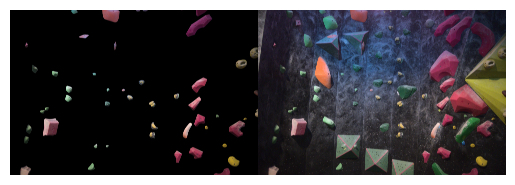
\includegraphics[width = \linewidth]{img/routes_std/big_cluster.jpg}
\caption{Histogram. One big cluster.}
\label{fig:big_cluster}
\end{figure}

\subsubsection{Learning-based approach} % Philipp
The problem of detecting a route on a climbing wall can be posed as a classification problem, e.g., given an image of a hold, assign it to its color.
Unfortunately, hold colors are not standardized between gyms, so one color can exist at one gym but not at the other. Furthermore, holds can also be multicolored, so this approach does not work in general.
We instead posed the problem as a similarity problem. Given two images of holds $x_1$, $x_2$ the model should learn if $x_1$ and $x_2$ belong to the same class (i.e. have the same color) or if they belong to different classes.


Our first implementation used a Siamese network \cite{Siamese} based on two pretrained Resnet50 \cite{Resnet} models with shared weights.
We used PyTorch \cite{Pytorch} to implement the model and used the pretrained weights from torchvision.
The classification layer was removed from the pretrained network, and we concatenated the output from the last layers. This was used as an input for multiple fully connected layers, with a final fully connected layer with an output dimension of 1. The output is mapped to $[0,1]$ using a Sigmoid activation function. A visualization of the model architecture can be seen in \autoref{fig:siamese}.

We train the model using a binary cross entropy loss, with AdamW \cite{AdamW} as an optimizer. The model is trained for 100 epochs with a learning rate of $\epsilon= 0.001$ without updating the weights of the ResNet model (i.e. only training the fully connected layers).
The ResNet weights are then unfrozen and trained for an additional 100 epochs, with a much smaller learning rate of $\epsilon= 0.00001$.
The holds are sampled by randomly selecting a training image that has route annotations. From this image, we randomly select a hold from a route, and then randomly select a hold that belongs to the same route or a different route. By fixing the image at the start of the sampling, we ensure that we do not accidentally pick a hold with the same color from a different route in the gym.

\begin{figure}
    \centering
    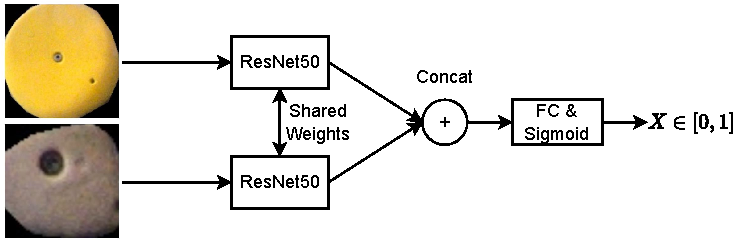
\includegraphics[width= \linewidth]{img/siamese_model.pdf}
    \caption{Siamese model example with two holds that are part of different routes.}
    \label{fig:siamese}
\end{figure}

Our second implementation is similar to FaceNet \cite{FaceNet}. Here, we use deep convolutional networks to learn embeddings such that the L2 distance between embeddings is small for holds that belong to the same route. Similar to the Siamese network, we use a pretrained Resnet50 model as base, with additional fully connected layers. The model embeds an image $x$ into a d-dimensional ($d=256$) vector space. Similar to \cite{FaceNet} we constrain the embedding such that $||f(x)||_{2} = 1$.
The model is trained by minimizing the triplet loss, which minimizes the distances between an anchor and a positive example, while maximizing the distance between the anchor and a negative example. A visualization of the triplet loss can be seen in \autoref{fig:triplet}.
Therefore we want
$$||a_{i} - p_{i}||_2 + \alpha < ||a_{i} - n_{i}||_2$$
where $\alpha$ is the margin between positive and negative pairs, and $a_i$, $p_i$, $n_i$ are the respective embeddings of the anchor, positive and negative images.
\begin{figure}
    \centering
    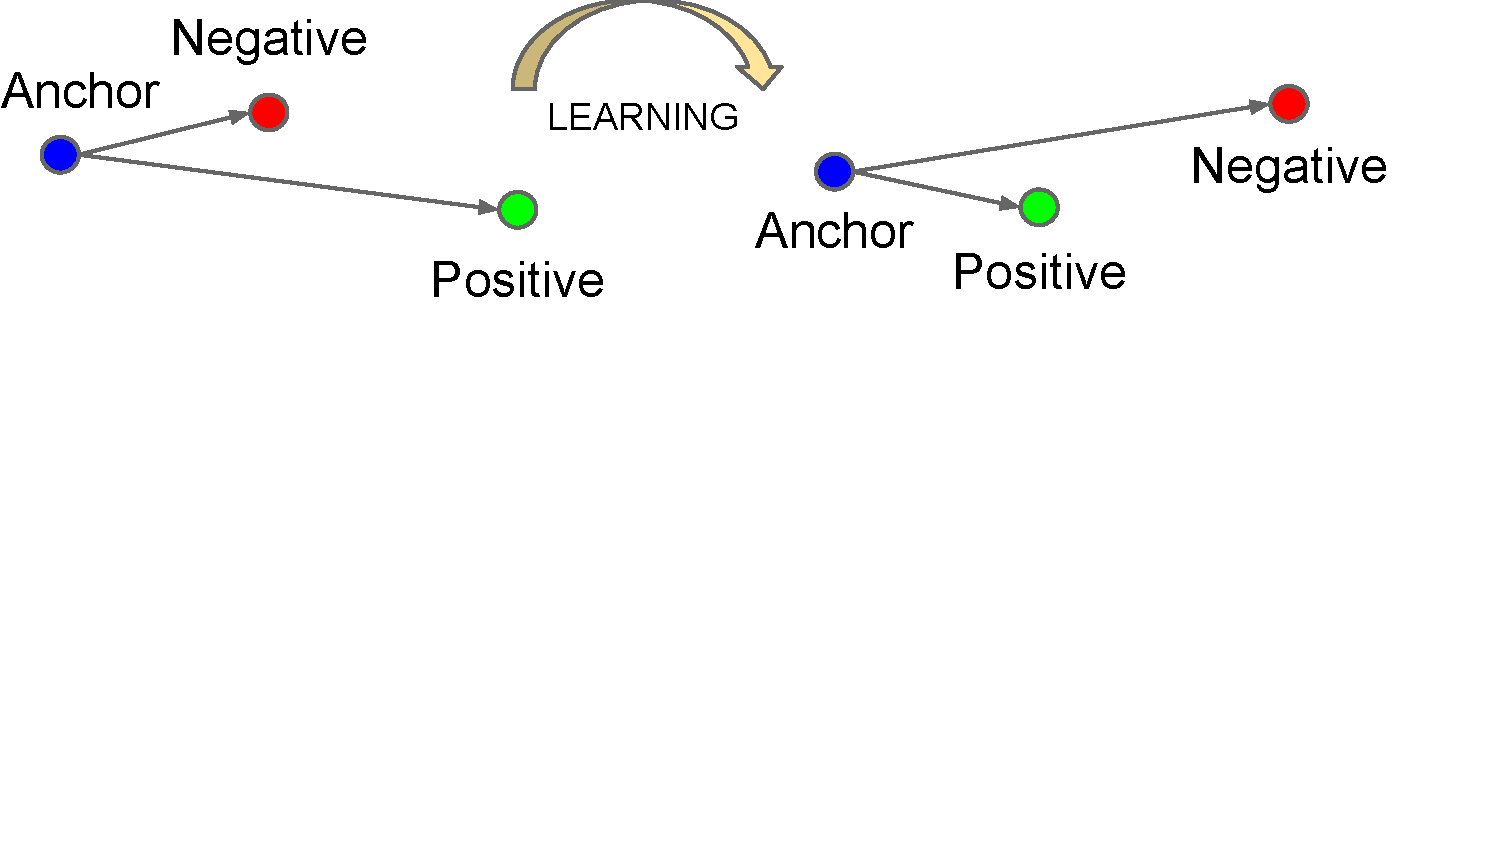
\includegraphics[trim=1cm 10cm 2.5cm 0cm, width = 0.9\linewidth]{img/triplet_viz.pdf}
    \caption{Triplet loss visualization \cite{FaceNet}.}
    \label{fig:triplet}
\end{figure}

The model is trained with the same hyperparameters as the Siamese network.
The sampling is done similar to the Siamese Network, instead we sample two pairs of the same route (anchor and positive example) and one image from a different route (negative example).
We experimented with triplet mining, i.e., identifying hard negative and hard positive triplets (triplets that violate the triplet constraint), in a mini-batch and using these to train the model. In theory, this should let the model converge faster because it is trained using difficult triplets and easier triplets are skipped. In our case, this only yielded minor improvements. A visualization of the triplet model can be seen in \autoref{fig:triplet_model}.

\begin{figure}
    \centering
    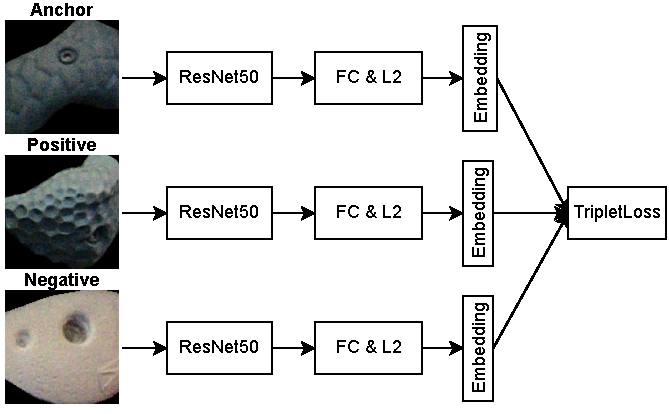
\includegraphics[width = 0.9\linewidth]{img/triplet_model.pdf}
    \caption{Triplet model visualization. Anchor and positive images are sampled from the same route, while negative images are sampled from a different route.}
    \label{fig:triplet_model}
\end{figure}

Similar to the learning based method for hold detection, we rely heavily on augmentations, because the number of labeled training images is quite limited. For both the Siamese and TripletNet we apply random rotations and horizontal and vertical flips to the input image. Furthermore, we do random color augmentations like changing the brightness, contrast, saturation or hue of the input images. For the color augmentations, we ensure that the same random augmentation is applied to each tuple or triplet of input images.

The Siamase model is evaluated by counting the number of random image tuples from the test dataset, where it correctly classifies that two images belong to the same or different route.
For the triplet model, we count the number of triplets where the embeddings of the anchor and positive image are closer together than the embedding of the anchor and negative image, i.e., the triplets where the triplet constraint $||a_i - p_i||_2 < ||a_i - n_i||_2$ holds.
The results of this evaluation can be seen in \autoref{tab:route_accuracy}.

\begin{table}[]
    \centering
    \begin{tabular}{lr}
    \toprule
         Model & Accuracy\\
         \midrule
         SiameseNet &  66.95\\
         TripletNet & 81.74\\ \bottomrule
    \end{tabular}
    \caption{Model accuracy for determining if two random holds belong to the same route or to different routes.}
    \label{tab:route_accuracy}
\end{table}

The route is then formed following a very simple algorithm. We initialize the first route by randomly picking a hold. Then we iterate over every hold in the image and calculate the distance between the current route-less hold and every hold in the existing route. If the median distance between the current hold and all holds in the existing route is smaller than a certain threshold $t_{\mathrm{med}}$ and the maximum distance is smaller than, $t_{\mathrm{max}}$ the hold is added to the existing route. This is repeated for all existing routes. If the hold is not similar to any holds on existing routes, a new route containing the hold is created.

The resulting routes can be seen in \autoref{fig:routes_ml}. As we can see from \autoref{fig:routes_ml:a} the routes from the SiameseNet are often too small, i.e., most of the holds in the detected route are of the same color, but it is missing several holds from the route and assigned them to another route.
The TripletNet creates much larger routes, often containing holds that have similar colors but belong to different routes, e.g., in \autoref{fig:routes_ml:b} light green and dark green holds are combined and even a couple of black-yellow holds are included. Similarly, in the pink cluster \autoref{fig:routes_ml:c} orange holds are included.
%The TripletNet creates much larger routes, most of which are the same color, e.g., in \autoref{fig:routes_ml:b} light green and dark green holds are combined and even a couple of black-yellow holds are included. Similarly, in the pink cluster \autoref{fig:routes_ml:c} orange holds are included.

\begin{figure}[t]
\centering
\begin{subfigure}{1\linewidth}
\centering
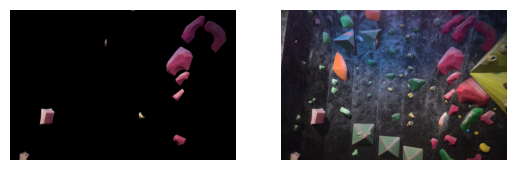
\includegraphics[width = \linewidth]{img/route_detection_ml/siamese_pink_cluster.png}
\caption{SiameseNet pink cluster}
\label{fig:routes_ml:a}
\end{subfigure}
\begin{subfigure}{1\linewidth}
\centering
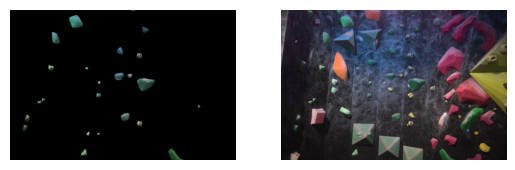
\includegraphics[width = \linewidth]{img/route_detection_ml/triplet_green_cluster.png}
\caption{TripletNet green cluster}
\label{fig:routes_ml:b}
\end{subfigure}
\begin{subfigure}{1\linewidth}
\centering
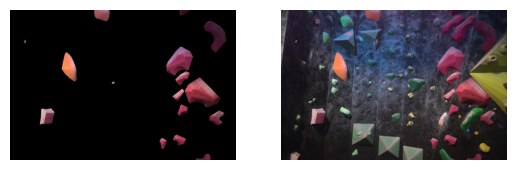
\includegraphics[width = \linewidth]{img/route_detection_ml/triplet_pink_cluster.png}
\caption{TripletNet pink cluster}
\label{fig:routes_ml:c}
\end{subfigure}
\begin{subfigure}{1\linewidth}
\centering
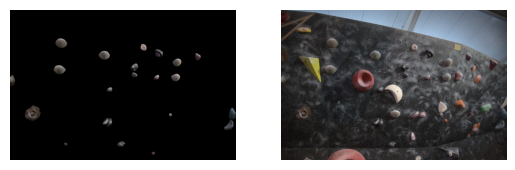
\includegraphics[width = \linewidth]{img/route_detection_ml/triplet_black_cluster.png}
\caption{TripletNet black/gray cluster}
\label{fig:routes_ml:d}
\end{subfigure}
\caption{Route detection hold clusters for SiameseNet and TripletNet. $t_{\mathrm{med}} = 0.7, t_{\mathrm{max}}=2.65$}
\label{fig:routes_ml}
\end{figure}


\section{Findings}

\subsection{Hold segmentation} % Tom + Philipp

Standard hold segmentation can only produce desirable results if the parameters are configured precisely for the given dataset and does not generalize well to changes in background and hold color.
While it does not require extensive manual image annotation like the learning-based approach, parameter tuning can be just as time-consuming and the results will likely be inferior.

Learning-based hold segmentation far outperforms the standard approach in terms of accuracy, but has a number of additional requirements, such as a CUDA-enabled GPU (for the majority of modern ML frameworks including ours), manual image annotation and training time.

\subsection{Route segmentation} % Kiryl
For standard route segmentation approach we found, that number of clusters have to be specified beforehand and Mean color clustering is supposed to be the most effective techniques we implemented for route segmentation.

The results of the machine learning approach for route segmentation are only slightly better than the standard route segmentation approach. The performance of the SiameseNet and TripletNet can probably be further improved by labeling more routes and training the model for a longer period of time. Another possible improvement could be the inclusion of the entire image in addition to the specific hold. This could let the model take spacial information into account in order to decide if two holds belong to the same route or a different route. 

\section{Conclusion} \label{sec:conclusion}

Standard and learning approaches were implemented for the task of hold and route segmentation.
For hold segmentation, the standard approach uses blob detection for detecting positions of holds and subsequent edge detection to find their contours, both implemented with OpenCV \cite{opencv}. The learning-based approach uses the detectron2 implementation of Mask R-CNN \cite{maskrcnn} which was fine-tuned to our task.

For route segmentation, the standard approach uses clustering via scikit-learn \cite{scikit}, also, image operations were done with OpenCV \cite{opencv}. Standard annotations were built on different feature sets like Mean colors, Histograms and Color moments. The learning-based approach uses a ResNet model to learn embeddings of holds, such that holds from the same route have a small L2 distance to each other.

In both of the tasks, the learning approach yields more accurate results, the tradeoff being the need to manually create an annotated dataset, which is the main factor driving the model accuracy.

The source code was made available free and open source under the GPLv3 license on GitHub: \url{https://github.com/xiaoxiae/Indoor-Climbing-Hold-and-Route-Segmentation}.
The dataset, including the best-performing models, can also be obtained under the CC BY-SA 4 license from Kaggle: \url{https://www.kaggle.com/datasets/tomasslama/indoor-climbing-gym-hold-segmentation}.
Two of the best performing models for hold and route segmentation were also released as a notebook on Kaggle and can thus be run online without the need for downloading anything: \url{https://www.kaggle.com/code/tomasslama/hold-segmentation/} and \url{https://www.kaggle.com/code/tomasslama/route-segmentation/}.

\section{Contributions}

Philipp:
\begin{itemize}
    \setlength\itemsep{0em}
    \item \textit{Work:} Dataset labeling, Dataset statistics, learning-based hold detection, standard route segmentation: Color moments \& Histogram, machine learning route segmentation (SiameseNet and TripleNet)
    \item \textit{Writing:} Learning-based hold detection, learning-based route segmentation (SiameseNet and TripletNet)
\end{itemize}

Tom: 
\begin{itemize}
    \setlength\itemsep{0em}
    \item \textit{Work:} Dataset labeling + photography, Dataset statistics/utility scripts, Standard hold detection, Kaggle
    \item \textit{Writing:} Abstract, Introduction, Method, Obtaining data, Standard hold approach, Hold segmentation findings, Conclusion
\end{itemize}

Kiryl:
\begin{itemize}
    \setlength\itemsep{0em}
    \item \textit{Work:} Standard route segmentation (Mean colors).
    \item \textit{Writing:} Standard route segmentation, Findings of standard route segmentation, Conclusion
\end{itemize}

{\small
\bibliographystyle{ieee_fullname}
\bibliography{egbib}
}

\end{document}
